\documentclass{beamer}
\mode<presentation>

% \documentclass[handout]{beamer}
% \mode<handout>{\setbeamercolor{background canvas}{bg=black!5}}
% \usepackage{pgfpages}
% \pgfpagesuselayout{2 on 1}[a4paper,border shrink=5mm]

\usepackage[T1]{fontenc}
\usepackage{tikz}
\usetikzlibrary {calc,graphs,graphs.standard,patterns.meta,intersections}
\usepackage{physics}
\usepackage{graphicx}
\usepackage{xcolor}
\definecolor{bgYellow}{HTML}{F0EBDC}
\definecolor{myViolet}{HTML}{403340}

\title{Origami Polyhedra}
\author[dishajk]{Disha Kuzhively\\{\scriptsize disha.jk@icts.res.in}\\ICTS-TIFR}
\institute{IISER Bhopal}
\date[IISER Bhopal]{20 and 21 November 2026}
\begin{document}
\setbeamercolor{background canvas}{bg=bgYellow}
\setbeamercolor{title}{fg=myViolet}
\setbeamercolor{frametitle}{fg=myViolet}
\addtobeamertemplate{footline}{}{%
    \hspace{1em}
    \textcolor{gray}{dishajk.github.io}
    \vspace{1em}
}
\begin{frame}
    \titlepage
\end{frame}
\begin{frame}
    \frametitle{Regular Polyhedra}
    \note{A polyhedron is a 3-dimensional solid whose boundry is made of polygonal faces.}
    \note{for a regular polyhedron, the faces are congruent regular polygons, and the same number of faces meet at every vertex.}
    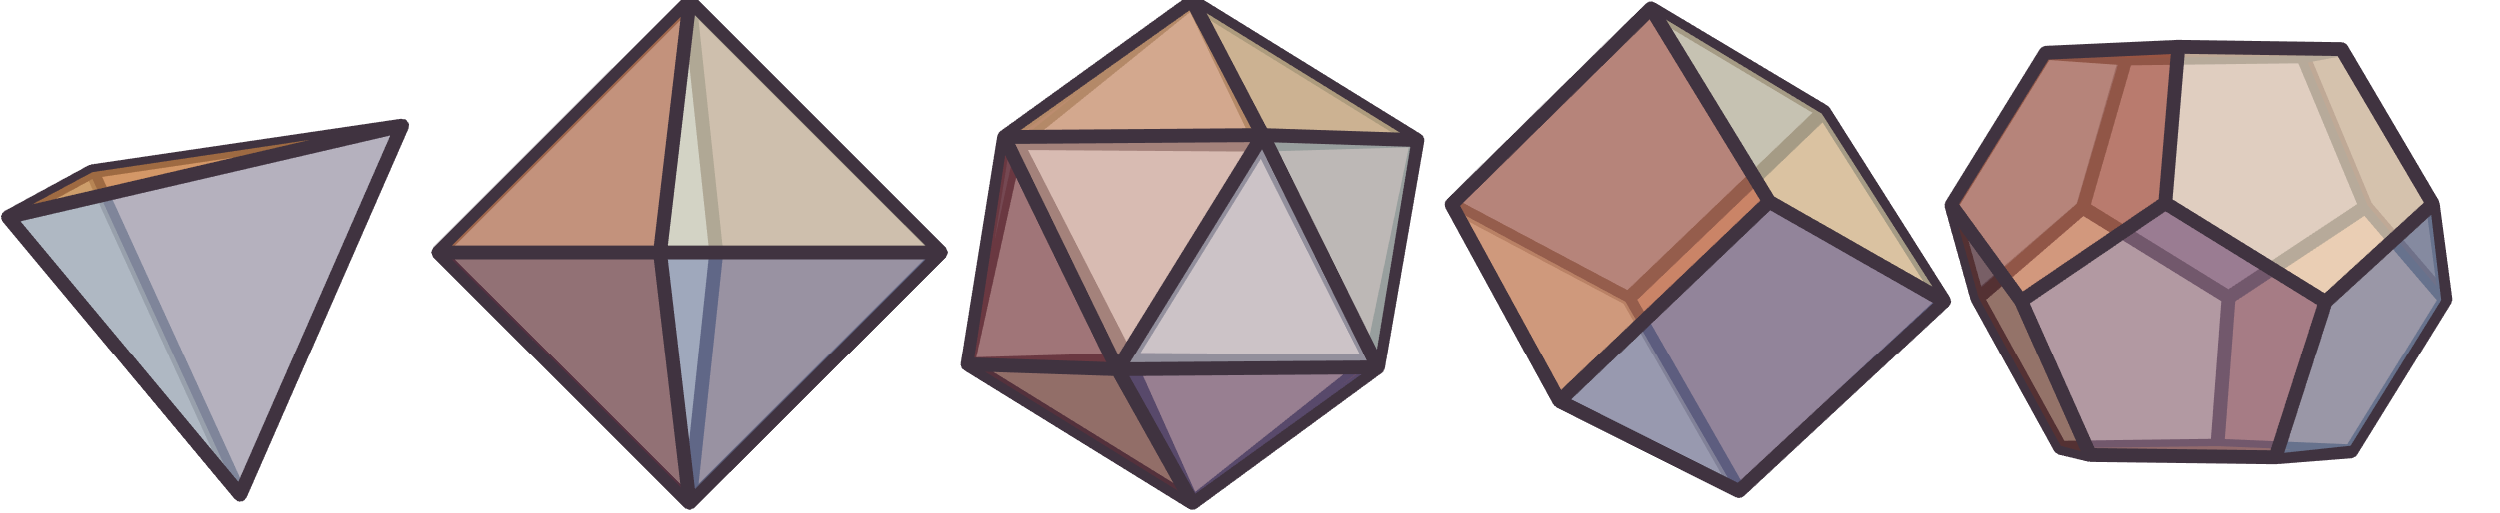
\includegraphics[width=\textwidth]{platonic}
    \note{question: only five types of regular polyhedra can exist, why?}
\end{frame}
\begin{frame}
    \only<2-14>{\frametitle{Triangle Unit}
    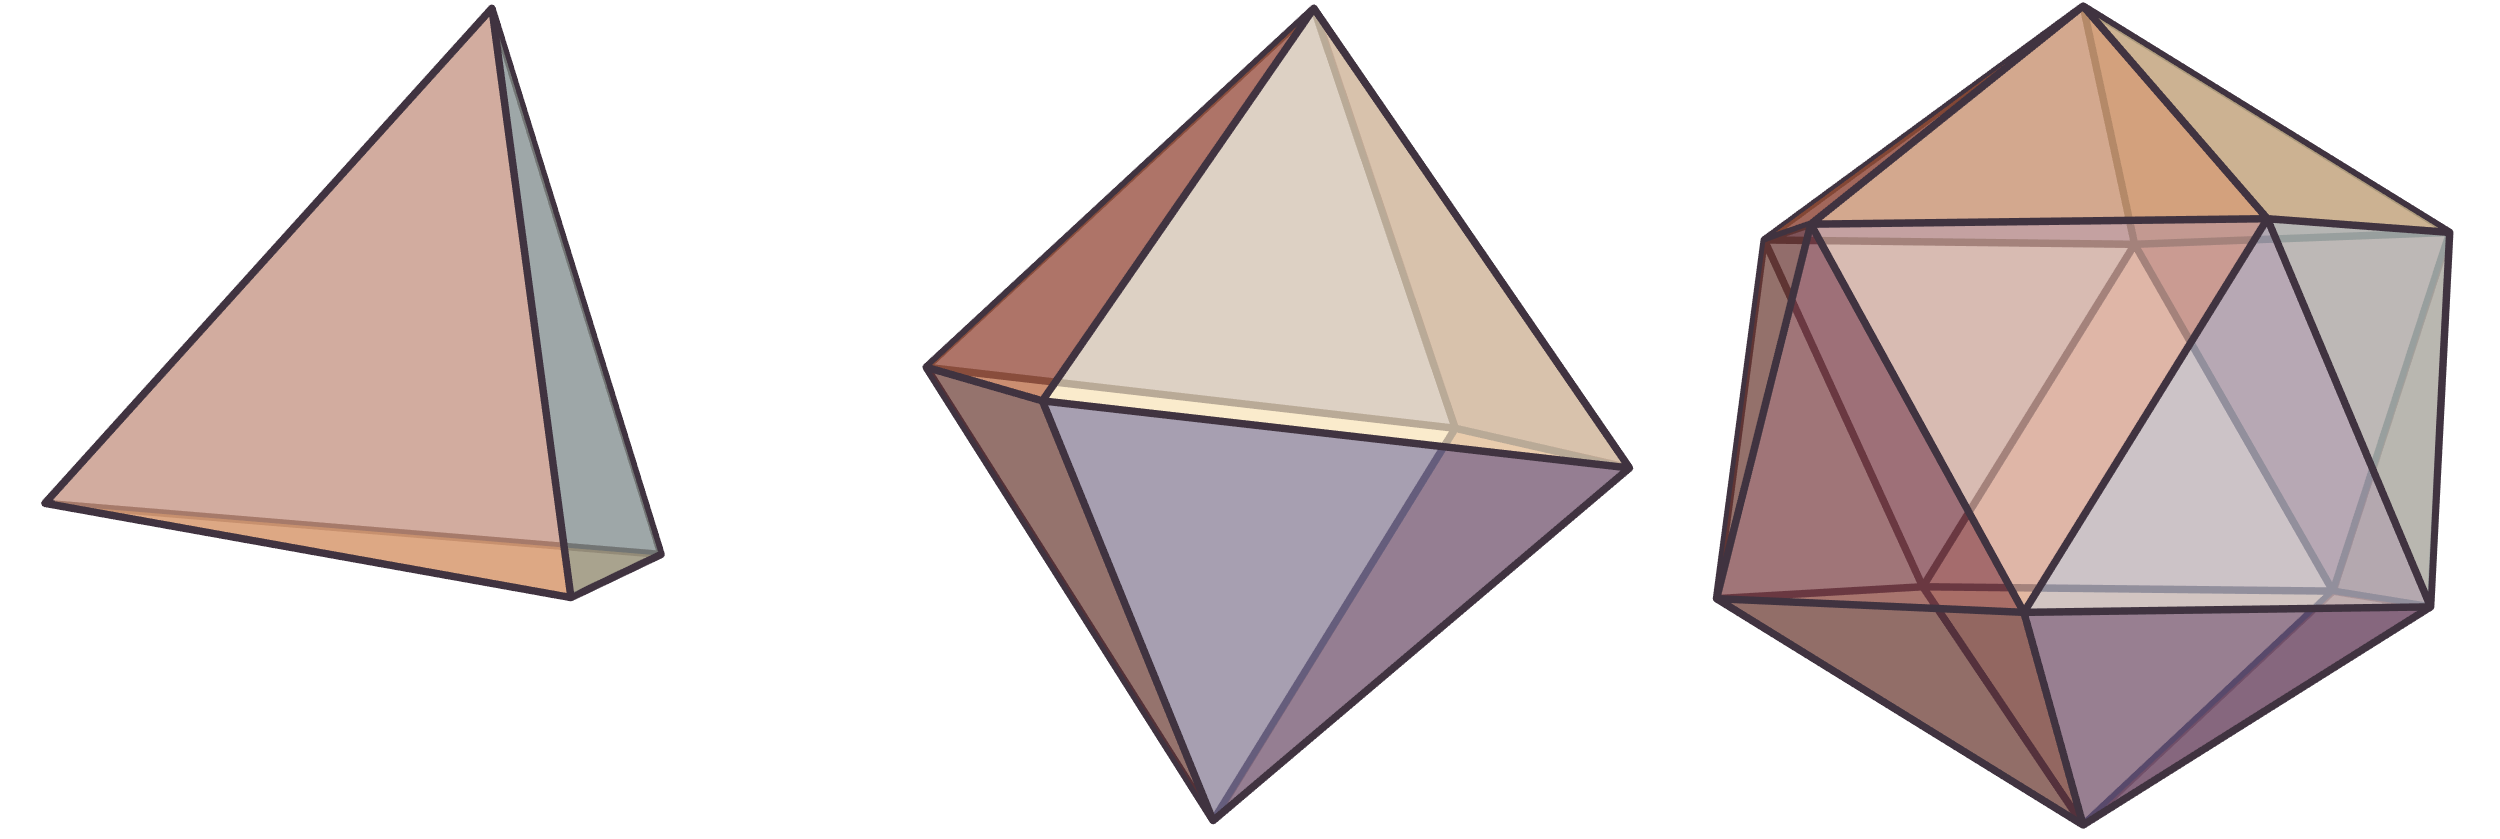
\includegraphics[height=0.1\textheight]{triplatonic}}
    \only<1>{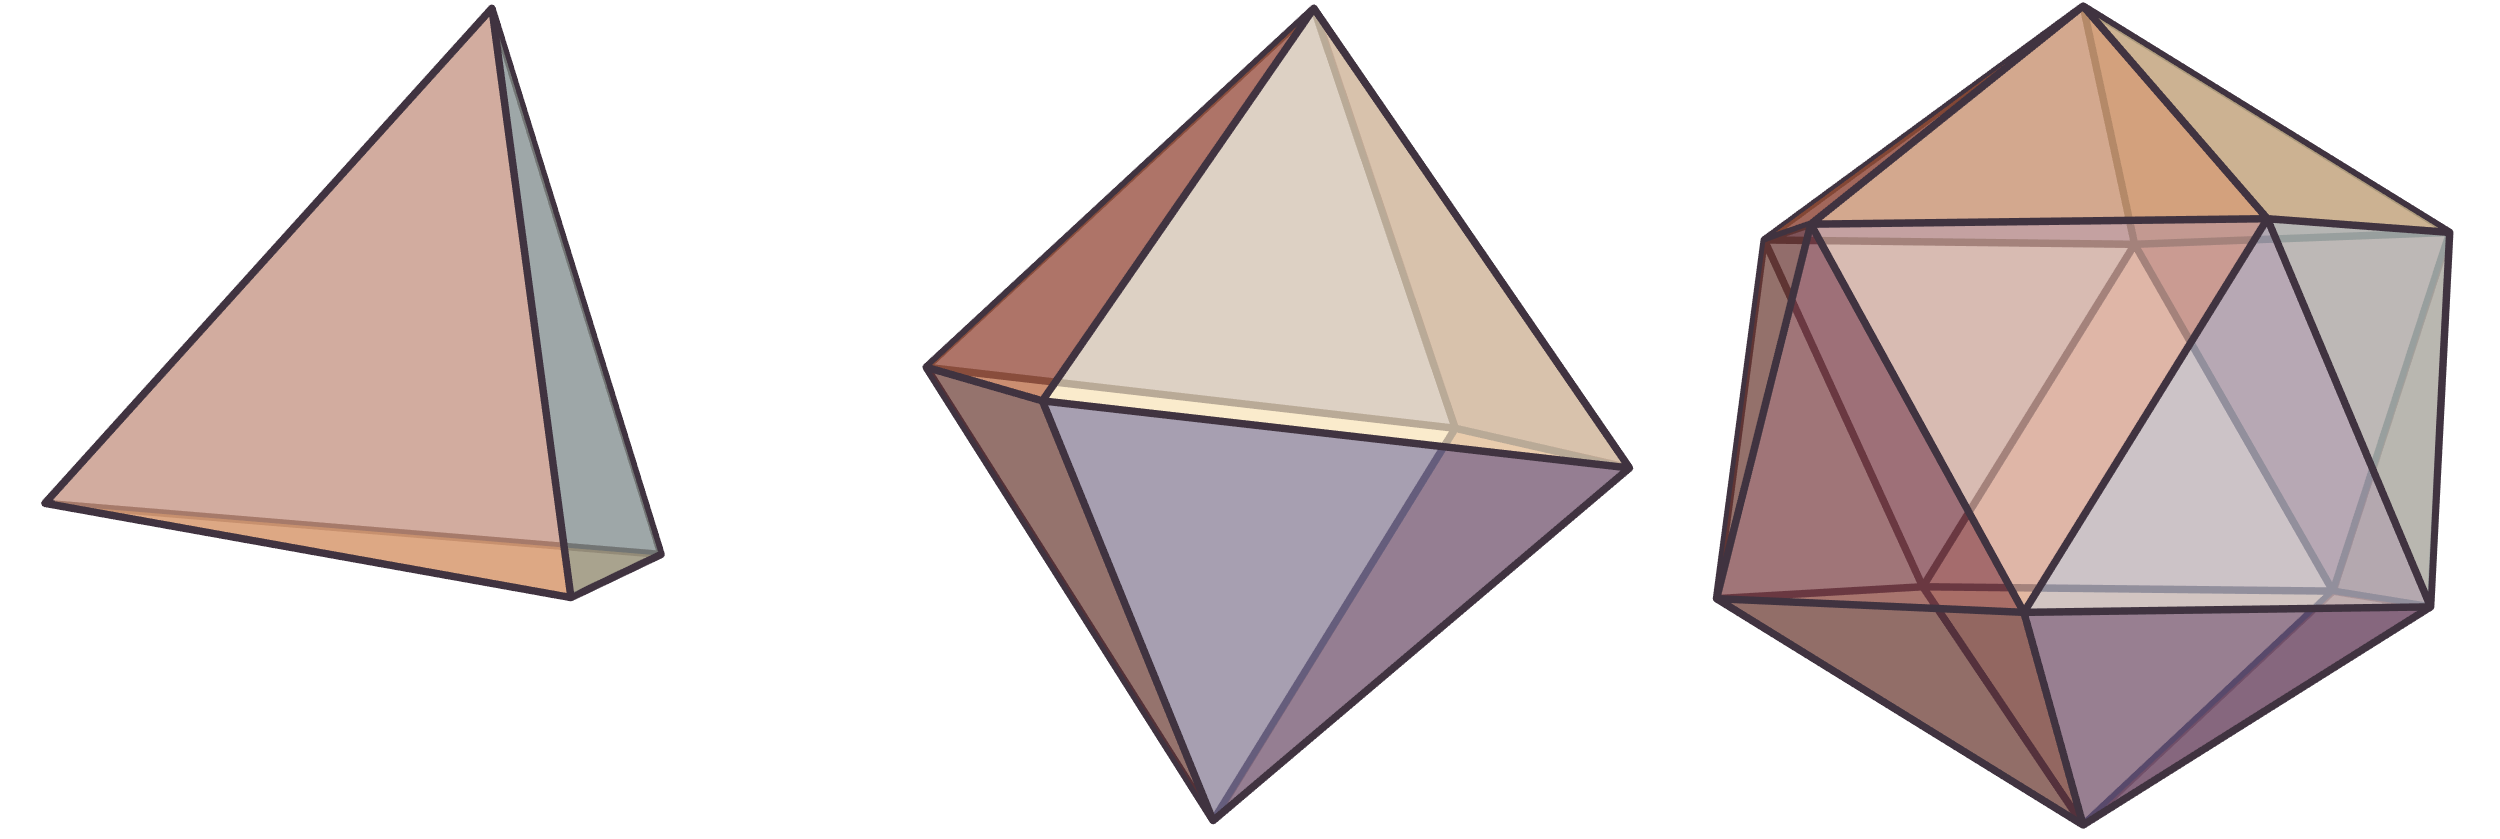
\includegraphics[width=\textwidth]{triplatonic}}

    \centering
    \begin{tikzpicture}
        \only<2-4,10>{
            \filldraw[white,draw=black] (0,0) rectangle (4,4);}
        \only<3-4,10>{
            \draw[dashed,thick] (2,0) -- (2,4);}
        \only<5>{
            \filldraw[white,draw=black,opacity=0.3] (0,0) rectangle (4,4);
            \draw[dashed,thick,opacity=0.3] (2,0) -- (2,4);
            \draw[dashed,thick,opacity=0.3] (0,2) -- (4,2);}
        \only<5-9>{
            \filldraw[gray!50,draw=black] (1,0) rectangle (3,4);
            \draw[thick,dotted] (1,2) -- (3,2);
            \draw[thick] (2,0) -- (2,4);}
        \only<11>{
            \filldraw[gray!50,draw=black,opacity=0.3] (0,0)     rectangle (4,{2-sqrt(3)});
            \filldraw[gray!50,draw=black,opacity=0.3] (0,{2+sqrt(3)})     rectangle (4,4);
            \draw[thick,dashed,opacity=0.3] (1,0) -- (1,{2-sqrt(3)});
            \draw[thick,dashed,opacity=0.3] (3,0) -- (3,{2-sqrt(3)});
            \draw[thick,dashed,opacity=0.3] (2,0) -- (2,{2-sqrt(3)});
            \draw[thick,dotted,opacity=0.3] (1,{2+sqrt(3)}) -- (1,4);
            \draw[thick,dotted,opacity=0.3] (2,{2+sqrt(3)}) -- (2,4);
            \draw[thick,dotted,opacity=0.3] (3,{2+sqrt(3)}) -- (3,4);
            }
        \only<11-12>{
            \filldraw[gray!50,draw=black] (0,{2-sqrt(3)})     rectangle (4,{4-2*sqrt(3)});
            \filldraw[gray!50,draw=black] (0,{2+sqrt(3)})     rectangle (4,{2*sqrt(3)});
            \filldraw[white,draw=black] (0,{4-2*sqrt(3)}) rectangle (4,{2*sqrt(3)});
            \draw[thick,dotted] (1,{2-sqrt(3)}) -- (1,{4-2*sqrt(3)});
            \draw[thick,dotted] (2,{2-sqrt(3)}) -- (2,{4-2*sqrt(3)});
            \draw[thick,dotted] (3,{2-sqrt(3)}) -- (3,{4-2*sqrt(3)});
            \draw[thick,dashed] (1,{4-2*sqrt(3)}) -- (1,{2*sqrt(3)});
            \draw[thick,dashed] (2,{4-2*sqrt(3)}) -- (2,{2*sqrt(3)});
            \draw[thick,dashed] (3,{4-2*sqrt(3)}) -- (3,{2*sqrt(3)});
            \draw[thick,dotted] (1,{2*sqrt(3)}) -- (1,{2+sqrt(3)});
            \draw[thick,dotted] (2,{2*sqrt(3)}) -- (2,{2+sqrt(3)});
            \draw[thick,dotted] (3,{2*sqrt(3)}) -- (3,{2+sqrt(3)});
            \draw[thick,dashed] (0,{2-sqrt(3)}) -- ({2/sqrt(3)-1},{4-2*sqrt(3)});
            \draw[thick,dotted] ({2/sqrt(3)-1},{4-2*sqrt(3)}) -- (1,2);
            \draw[thick,dashed] (0,{2+sqrt(3)}) -- ({2/sqrt(3)-1},{2*sqrt(3)});
            \draw[thick,dotted] ({2/sqrt(3)-1},{2*sqrt(3)}) -- (1,2);
            \draw[thick,dashed] (4,{2-sqrt(3)}) -- ({5-2/sqrt(3)},{4-2*sqrt(3)});
            \draw[thick,dotted] ({5-2/sqrt(3)},{4-2*sqrt(3)}) -- (3,2);
            \draw[thick,dashed] (4,{2+sqrt(3)}) -- ({5-2/sqrt(3)},{2*sqrt(3)});
            \draw[thick,dotted] ({5-2/sqrt(3)},{2*sqrt(3)}) -- (3,2);
            \draw[thick,dotted] (2,{2+sqrt(3)}) -- ({3-2/sqrt(3)},{2*sqrt(3)});
            \draw[thick,dashed] ({3-2/sqrt(3)},{2*sqrt(3)}) -- (1,2);
            \draw[thick,dotted] (2,{2-sqrt(3)}) -- ({3-2/sqrt(3)},{4-2*sqrt(3)});
            \draw[thick,dashed] ({3-2/sqrt(3)},{4-2*sqrt(3)}) -- (1,2);
            \draw[thick,dotted] (2,{2+sqrt(3)}) -- ({1+2/sqrt(3)},{2*sqrt(3)});
            \draw[thick,dashed] ({1+2/sqrt(3)},{2*sqrt(3)})--(3,2);
            \draw[thick,dotted] (2,{2-sqrt(3)}) -- ({1+2/sqrt(3)},{4-2*sqrt(3)});
            \draw[thick,dotted] ({1+2/sqrt(3)},{4-2*sqrt(3)})--(3,2);
            }
        \only<6-12>{
            \draw[thick,dashed] (1,3) -- (3,3);
            \draw[thick,dashed] (1,1) -- (3,1);}
        \only<7>{
            \filldraw[gray!15] (1,2) -- ({1+2/sqrt(3)},4)--(1,4)--cycle;
            \filldraw[gray!50,draw=black] (1,2) -- ({1+sqrt(3)},3)--({1+2/sqrt(3)},4)--cycle;
            \draw[thick,dotted]  ({1+1/sqrt(3)},3)--(2,{2+1/sqrt(3)});
        }
        \only<8-10>{
            \draw[thick,dashed] (1,2) -- ({1+2/sqrt(3)},4);
        }
        \only<9-10>{
            \draw[thick,dashed] (1,2) -- ({1+2/sqrt(3)},0);
            \draw[thick,dashed] (3,2) -- ({3-2/sqrt(3)},0);
            \draw[thick,dashed] (3,2) -- ({3-2/sqrt(3)},4);
        }
        \only<10>{
            \draw[thick,dashed] (1,0) -- (1,4);    
            \draw[thick,dashed] (3,0) -- (3,4);
            \draw[thick,dotted] (0,{2+sqrt(3)}) -- ({2/sqrt(3)-1},4);
            \draw[thick,dotted] (4,{2+sqrt(3)}) -- ({5-2/sqrt(3)},4);
            \draw[thick,dotted] (0,{2-sqrt(3)}) -- ({2/sqrt(3)-1},0);
            \draw[thick,dotted] (4,{2-sqrt(3)}) -- ({5-2/sqrt(3)},0);     
        }
        \only<4,10-12>{
            \draw[dashed,thick] (0,2) -- (4,2);}
        \only<10>{
            \draw[thick,dotted] (0,{2-sqrt(3)}) -- (1,2);
            \draw[thick,dotted] (0,{2+sqrt(3)}) -- (1,2);
            \draw[thick,dotted] (4,{2-sqrt(3)}) -- (3,2);
            \draw[thick,dotted] (4,{2+sqrt(3)}) -- (3,2);
        }
        \only<10-12>{
            \draw[thick,dotted] (0,3) -- (1,3);
            \draw[thick,dotted] (0,1) -- (1,1);
            \draw[thick,dotted] (3,3) -- (4,3);
            \draw[thick,dotted] (3,1) -- (4,1);
        }
        \only<12>{
            \filldraw[gray!15] (0,2) -- (1,{2+sqrt(3)}) -- (0,{2+sqrt(3)})--cycle;
            \filldraw[gray!15] (4,2) -- (3,{2-sqrt(3)}) -- (4,{2-sqrt(3)})--cycle;
            \filldraw[gray!50,draw=black] (0,2) -- (1,{2+sqrt(3)})-- ({3/2},{2+sqrt(3)/2})--cycle;
            \draw[thick,dashed] ({3/2},{2+sqrt(3)/2}) -- ({1/2},{2+sqrt(3)/2});
            \draw[thick,dashed] ({1/sqrt(3)},3) -- ({sqrt(3)/2},{5/2});
            \filldraw[gray!50,draw=black] (4,2) -- (3,{2-sqrt(3)})-- ({5/2},{2-sqrt(3)/2})--cycle;
            \draw[thick,dashed] ({5/2},{2-sqrt(3)/2}) -- ({7/2},{2-sqrt(3)/2});
            \draw[thick,dashed] ({4-1/sqrt(3)},1) -- ({4-sqrt(3)/2},{3/2});
        }
        \only<12>{
            \filldraw[xshift=5cm,gray!50,draw=black] (0,{2-sqrt(3)})     rectangle (4,{4-2*sqrt(3)});
            \filldraw[xshift=5cm,gray!50,draw=black] (0,{2+sqrt(3)})     rectangle (4,{2*sqrt(3)});
            \filldraw[xshift=5cm,white,draw=black] (0,{4-2*sqrt(3)}) rectangle (4,{2*sqrt(3)});
            \draw[xshift=5cm,thick,dotted] (1,{2-sqrt(3)}) -- (1,{4-2*sqrt(3)});
            \draw[xshift=5cm,thick,dotted] (2,{2-sqrt(3)}) -- (2,{4-2*sqrt(3)});
            \draw[xshift=5cm,thick,dotted] (3,{2-sqrt(3)}) -- (3,{4-2*sqrt(3)});
            \draw[xshift=5cm,thick,dashed] (1,{4-2*sqrt(3)}) -- (1,{2*sqrt(3)});
            \draw[xshift=5cm,thick,dashed] (2,{4-2*sqrt(3)}) -- (2,{2*sqrt(3)});
            \draw[xshift=5cm,thick,dashed] (3,{4-2*sqrt(3)}) -- (3,{2*sqrt(3)});
            \draw[xshift=5cm,thick,dotted] (1,{2*sqrt(3)}) -- (1,{2+sqrt(3)});
            \draw[xshift=5cm,thick,dotted] (2,{2*sqrt(3)}) -- (2,{2+sqrt(3)});
            \draw[xshift=5cm,thick,dotted] (3,{2*sqrt(3)}) -- (3,{2+sqrt(3)});
            \draw[xshift=5cm,thick,dashed] (0,{2-sqrt(3)}) -- ({2/sqrt(3)-1},{4-2*sqrt(3)});
            \draw[xshift=5cm,thick,dotted] ({2/sqrt(3)-1},{4-2*sqrt(3)}) -- (1,2);
            \draw[xshift=5cm,thick,dashed] (0,{2+sqrt(3)}) -- ({2/sqrt(3)-1},{2*sqrt(3)});
            \draw[xshift=5cm,thick,dotted] ({2/sqrt(3)-1},{2*sqrt(3)}) -- (1,2);
            \draw[xshift=5cm,thick,dashed] (4,{2-sqrt(3)}) -- ({5-2/sqrt(3)},{4-2*sqrt(3)});
            \draw[xshift=5cm,thick,dotted] ({5-2/sqrt(3)},{4-2*sqrt(3)}) -- (3,2);
            \draw[xshift=5cm,thick,dashed] (4,{2+sqrt(3)}) -- ({5-2/sqrt(3)},{2*sqrt(3)});
            \draw[xshift=5cm,thick,dotted] ({5-2/sqrt(3)},{2*sqrt(3)}) -- (3,2);
            \draw[xshift=5cm,thick,dotted] (2,{2+sqrt(3)}) -- ({3-2/sqrt(3)},{2*sqrt(3)});
            \draw[xshift=5cm,thick,dashed] ({3-2/sqrt(3)},{2*sqrt(3)}) -- (1,2);
            \draw[xshift=5cm,thick,dotted] (2,{2-sqrt(3)}) -- ({3-2/sqrt(3)},{4-2*sqrt(3)});
            \draw[xshift=5cm,thick,dashed] ({3-2/sqrt(3)},{4-2*sqrt(3)}) -- (1,2);
            \draw[xshift=5cm,thick,dotted] (2,{2+sqrt(3)}) -- ({1+2/sqrt(3)},{2*sqrt(3)});
            \draw[xshift=5cm,thick,dashed] ({1+2/sqrt(3)},{2*sqrt(3)})--(3,2);
            \draw[xshift=5cm,thick,dotted] (2,{2-sqrt(3)}) -- ({1+2/sqrt(3)},{4-2*sqrt(3)});
            \draw[xshift=5cm,thick,dotted] ({1+2/sqrt(3)},{4-2*sqrt(3)})--(3,2);
            \draw[xshift=5cm,dashed,thick] (0,2) -- (4,2);
            \draw[xshift=5cm,thick,dashed] (1,3) -- (3,3);
            \draw[xshift=5cm,thick,dashed] (1,1) -- (3,1);
            \draw[xshift=5cm,thick,dotted] (0,3) -- (1,3);
            \draw[xshift=5cm,thick,dotted] (0,1) -- (1,1);
            \draw[xshift=5cm,thick,dotted] (3,3) -- (4,3);
            \draw[xshift=5cm,thick,dotted] (3,1) -- (4,1);
            \filldraw[xshift=5cm,gray!15] (0,2) -- (1,{2-sqrt(3)}) -- (0,{2-sqrt(3)})--cycle;
            \filldraw[xshift=5cm,gray!15] (4,2) -- (3,{2+sqrt(3)}) -- (4,{2+sqrt(3)})--cycle;
            \filldraw[xshift=5cm,gray!50,draw=black] (0,2) -- (1,{2-sqrt(3)})-- ({3/2},{2-sqrt(3)/2})--cycle;
            \draw[xshift=5cm,thick,dashed] ({3/2},{2-sqrt(3)/2}) -- ({1/2},{2-sqrt(3)/2});
            \draw[xshift=5cm,thick,dashed] ({1/sqrt(3)},1) -- ({sqrt(3)/2},{3/2});
            \filldraw[xshift=5cm,gray!50,draw=black] (4,2) -- (3,{2+sqrt(3)})-- ({5/2},{2+sqrt(3)/2})--cycle;
            \draw[xshift=5cm,thick,dashed] ({5/2},{2+sqrt(3)/2}) -- ({7/2},{2+sqrt(3)/2});
            \draw[xshift=5cm,thick,dashed] ({4-1/sqrt(3)},3) -- ({4-sqrt(3)/2},{5/2});
        }
        \only<13>{
            \filldraw[gray!15] (0,{2-sqrt(3)}) -- (0,2) -- (1,{2+sqrt(3)}) -- (4,{2+sqrt(3)}) -- (4,2) -- (3,{2-sqrt(3)}) -- cycle;}
        \only<13-14>{
            \filldraw[white,draw=black] (0,{2-sqrt(3)}) -- (2,{2-sqrt(3)}) --(4,{2+sqrt(3)}) -- (2,{2+sqrt(3)})--cycle;
        }
         \only<13-14>{
            \filldraw[gray!50,draw=black] (0,{2-sqrt(3)}) -- (2,{2-sqrt(3)}) -- ({1+2/sqrt(3)},{4-2*sqrt(3)}) -- ({2/sqrt(3)-1},{4-2*sqrt(3)}) -- cycle;
            \filldraw[gray!50,draw=black] (2,{2+sqrt(3)}) -- (4,{2+sqrt(3)}) -- ({5-2/sqrt(3)},{2*sqrt(3)}) -- ({3-2/sqrt(3)},{2*sqrt(3)}) -- cycle;
            \filldraw[gray!50,draw=black] (0,{2-sqrt(3)}) -- ({3/2},{2-sqrt(3)/2})--({5/2},{2+sqrt(3)/2}) -- (2,{2+sqrt(3)}) -- cycle;
            \filldraw[gray!50,draw=black] (2,{2-sqrt(3)}) -- ({3/2},{2-sqrt(3)/2})--({5/2},{2+sqrt(3)/2}) -- (4,{2+sqrt(3)}) -- cycle;
        }
         \only<13>{
            \filldraw[xshift=5cm,gray!15] (1,{2-sqrt(3)}) -- (0,2) -- (0,{2+sqrt(3)}) -- (3,{2+sqrt(3)}) -- (4,2) -- (4,{2-sqrt(3)}) -- cycle;}
        \only<13-14>{
            \filldraw[xshift=5cm,white,draw=black] (2,{2-sqrt(3)}) -- (4,{2-sqrt(3)}) --(2,{2+sqrt(3)}) -- (0,{2+sqrt(3)})--cycle;
        }
         \only<13-14>{
            \filldraw[xshift=5cm,gray!50,draw=black] (0,{2+sqrt(3)}) -- (2,{2+sqrt(3)}) -- ({1+2/sqrt(3)},{2*sqrt(3)}) -- ({2/sqrt(3)-1},{2*sqrt(3)}) -- cycle;
            \filldraw[xshift=5cm,gray!50,draw=black] (2,{2-sqrt(3)}) -- (4,{2-sqrt(3)}) -- ({5-2/sqrt(3)},{4-2*sqrt(3)}) -- ({3-2/sqrt(3)},{4-2*sqrt(3)}) -- cycle;
            \filldraw[xshift=5cm,gray!50,draw=black] (4,{2-sqrt(3)}) -- ({5/2},{2-sqrt(3)/2})--({3/2},{2+sqrt(3)/2}) -- (2,{2+sqrt(3)}) -- cycle;
            \filldraw[xshift=5cm,gray!50,draw=black] (2,{2-sqrt(3)}) -- ({5/2},{2-sqrt(3)/2})--({3/2},{2+sqrt(3)/2}) -- (0,{2+sqrt(3)}) -- cycle;
        }
        \only<14>{
            \draw[thick,dotted] (2,{2-sqrt(3)}) -- (1,2) -- (3,2) -- (2,{2+sqrt(3)});
        }
        \only<14>{
            \draw[xshift=5cm,thick,dotted] (2,{2-sqrt(3)}) -- (3,2) -- (1,2) -- (2,{2+sqrt(3)});
        }
    \end{tikzpicture}

    \only<2>{Take a square piece of paper.}  
    \only<3>{Fold in half horizontally, crease, and unfold.}
    \only<4>{Fold in half vertically, crease, and unfold.}
    \only<5>{Fold the left and right sides to the middle.}
    \only<6>{Fold the top and bottom sides to the center, crease, and unfold.}
    \only<7>{Fold the top left corner to touch the line dividing the top half.}
    \only<8>{Crease and unfold.}
    \only<9>{Repeat the same for each of the other corners.}
    \only<10>{Unfold the paper.}
    \only<11>{Fold over the top and bottom edges along a line which passes through the points where the creases near the top and bottom of the paper cross.}
    \only<12>{Fold along the diagonals of the top (bottom) left and bottom (top) right rectangles.}
    \only<13>{Fold along the diagonals of the left and right rectangle.}
    \only<14>{Crease the triangles.\cite{verrillOrigami}}
\end{frame}
\begin{frame}
    \only<2-9>{\frametitle{Sonobe Unit}
    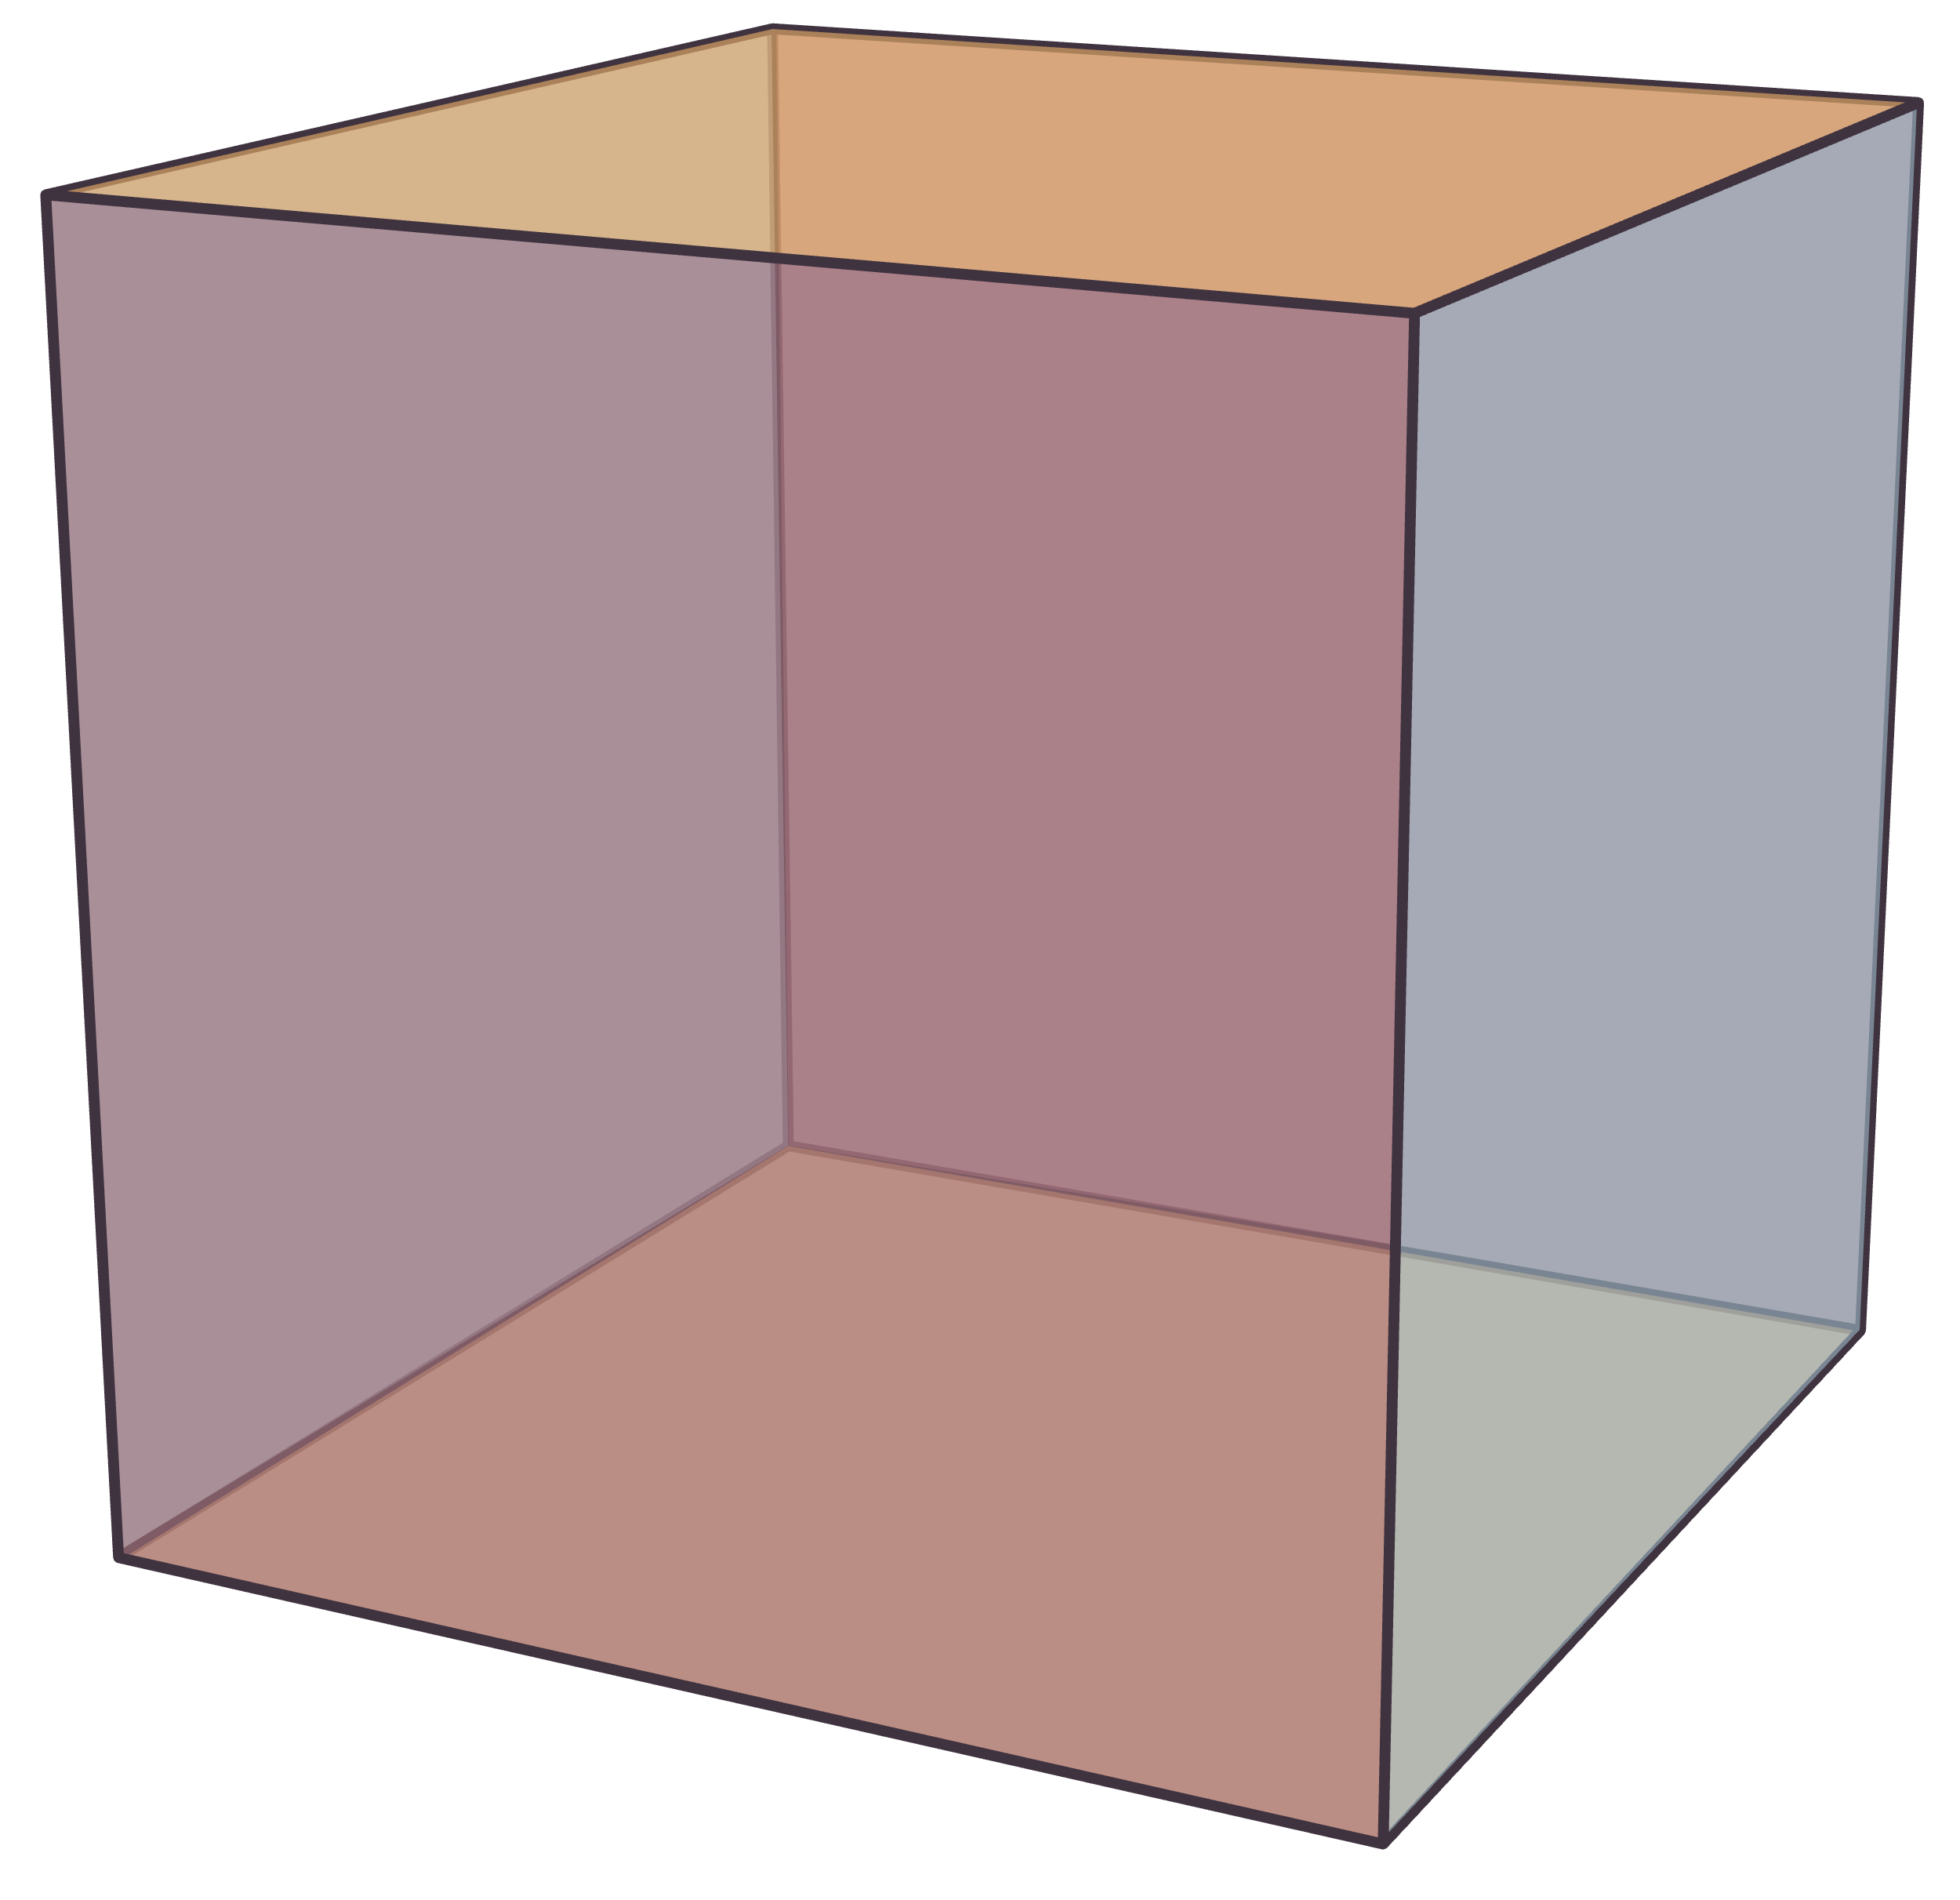
\includegraphics[height=0.1\textheight]{cube}}
    \only<1>{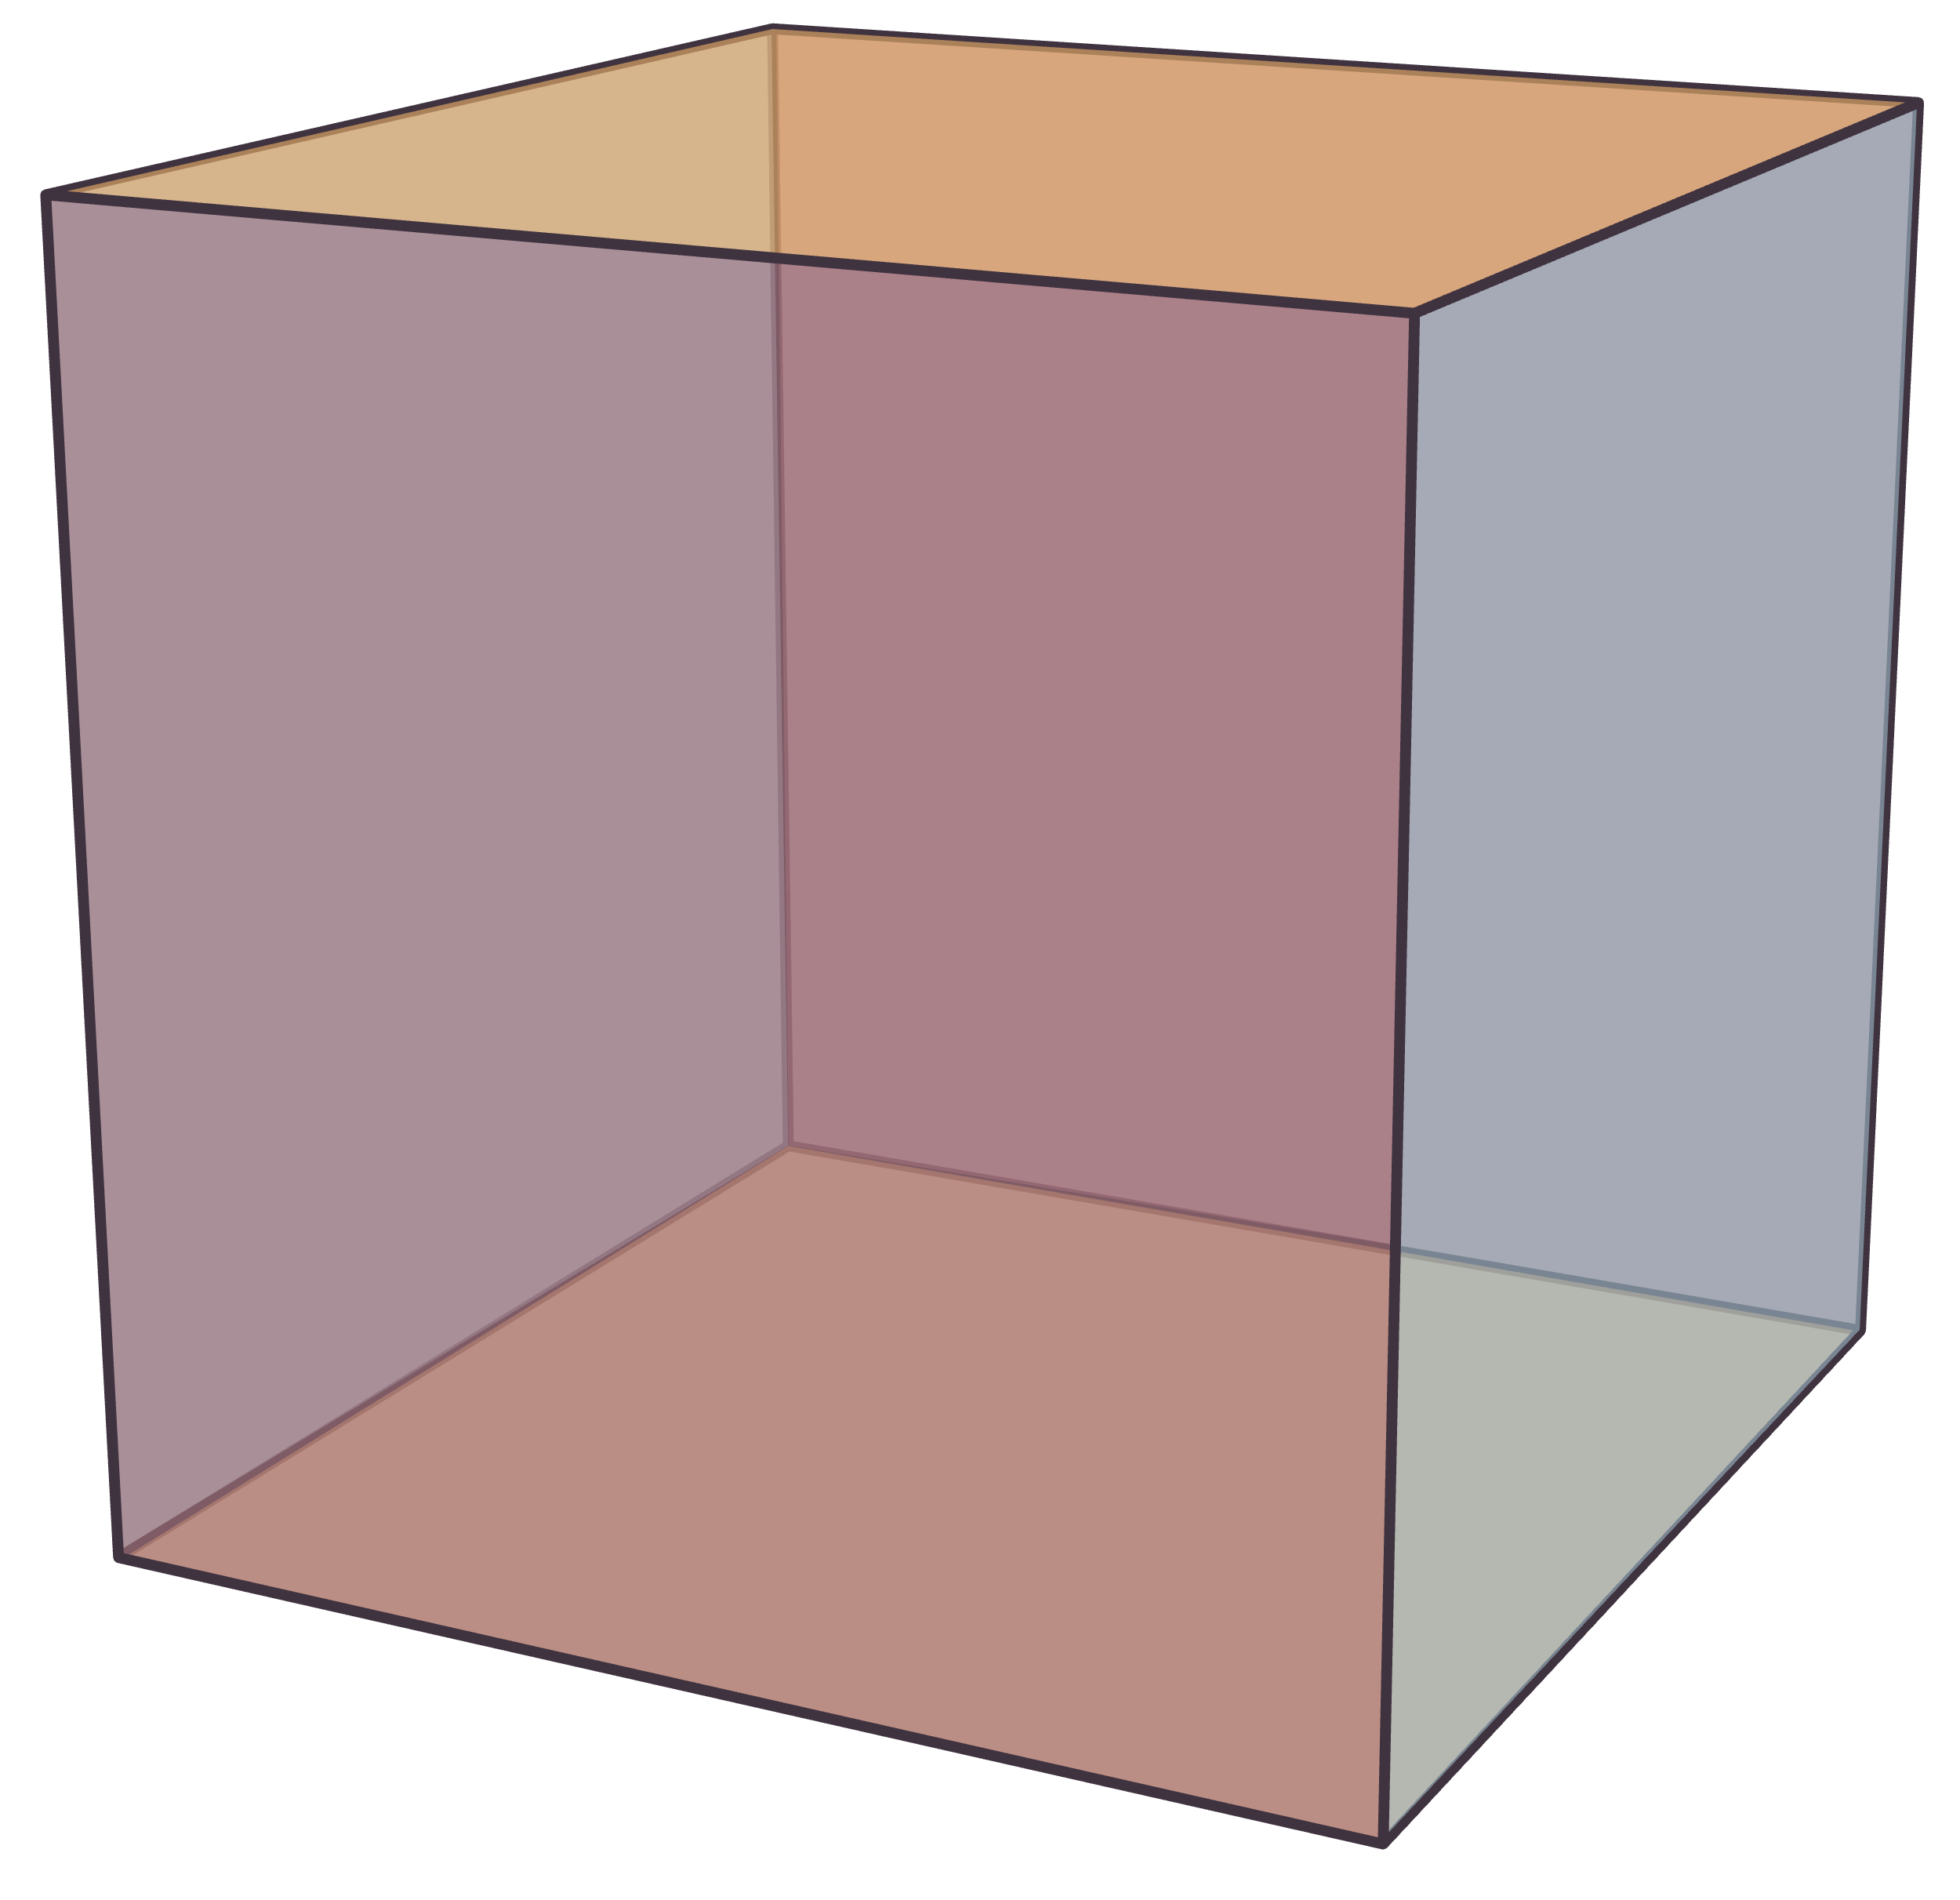
\includegraphics[height=0.7\textheight]{cube}}

    \centering
    \begin{tikzpicture}
    \only<2-3>{\draw[thick] (0,0) rectangle (4,4);}
    \only<2-5>{
    \draw[dashed] (0,2) -- (4,2);}
    \only<2-4>{
    \draw[dashed] (2,0) -- (2,4);}
    \only<2>{
    \draw[->] (2, 4) to[out=180,in=180] (2, 0);
    \draw[->] (0, 2) to[out=90,in=90] (4, 2);}
    \only<3-5>{
    \draw[dashed] (0,3) -- (4,3);
    \draw[dashed] (0,1) -- (4,1);}
    \only<3>{
    \draw[->] (1, 4) to[out=180,in=180] (1, 2);
    \draw[->] (3, 0) to[out=0,in=0] (3, 2);
    }
    \only<4>{
    \draw[thick] (0,0) --(3,0) -- (3,1) --(4,1) -- (4,4) -- (1,4) --(1,3) --(0,3) --(0,0);
    \fill[black, opacity=0.3] (0,3) -- (1,3) -- (1,4) -- cycle;
    \draw[->] (0.5, 3.75) to[out=180,in=180] (0.5, 3.25);
    \draw[->] (3.5, 0.25) to[out=0,in=0] (3.5, 0.75);}
    \only<4-5>{
    \fill[black, opacity=0.3] (3,0) -- (4,1) -- (3,1) -- cycle;
    }
    \only<5>{
    \draw[thick] (0,3) -- (0,0) --(3,0) -- (3,1) --(4,1) -- (4,3);
    \draw[thick] (1,2) -- (4,2);
    \fill[black, opacity=0.3] (0,3) -- (1,2) -- (4,2) -- (4,3) -- cycle;
    \draw[->] (2, 3.25) to[out=180,in=180] (2, 2.75);}
    \only<5-6>{
    \draw[dashed] (2,0) -- (2,2);
    \draw (3,0) -- (4,1);}
    \only<5-7>{
    \draw (0,3) -- (1,2);}
    \only<6>{
    \draw[thick] (0,3) -- (0,0) --(3,0) -- (3,1) --(4,1) -- (2,1);
    \fill[black, opacity=0.3] (0,3) -- (1,2) -- (2,2) -- (2,1) -- (3,1) --(3,0) -- (4,1) -- (2,3) --cycle;
    \draw[dashed] (0,2) -- (2,2);
    \draw (0,3) -- (2,3) -- (2,1);
    \draw[dashed] (0,1) -- (4,1);
    \draw[->] (3, 2.5) to[out=0,in=0] (3, 1.5);
    }
    \only<6-8>{
    \draw[thick] (1,2) -- (2,2);
    }
    \only<7>{
    \fill[black, opacity=0.3] (0,3) -- (1,2) -- (0,2) -- (0,1) -- (4,1) -- (2,3) -- cycle;
    \draw (0,3) -- (2,3) -- (2,2);
    \draw (2,3) -- (4,1);
    \draw[->] (2, 0.5) to[out=0,in=0] (2, 1.5);
    }
    \only<7-8>{
    \draw[thick] (0,3) -- (0,1) -- (0,2) -- (3,2);}
    \only<8>{
    \fill[black, opacity=0.3] (0,3) -- (1,2.1) -- (2,2) -- (0,2) -- (0,1) -- (4,1) -- (2,3) -- cycle;
    \draw[dashed] (1,2) -- (2,2);
    \draw (0,3) -- (2,3) -- (2,2);
    \draw (2,3) -- (4,1) -- (0,1);
    \draw[->] (0,1) to[out=180,in=190] (0.5, 2.5);
    \draw (0,3) -- (1,2.1) -- (2,2);
    }
    \only<9>{
    \fill[black, opacity=0.3] (0,3) -- (2,1)-- (4,1) -- (2,3) -- cycle;
    \draw[thick] (1,2) -- (3,2);
    \draw (0,3) -- (2,3) -- (2,2);
    \draw (2,3) -- (4,1) -- (2,1);
    \draw (0,3) -- (2,1) -- (2,2);
    \draw[dotted] (1,2) -- (2,3);
    \draw[dotted] (2,1) -- (3,2);
    }
\end{tikzpicture}
\end{frame}
\begin{frame}
    \only<2-16>{\frametitle{Pentagon Unit}
    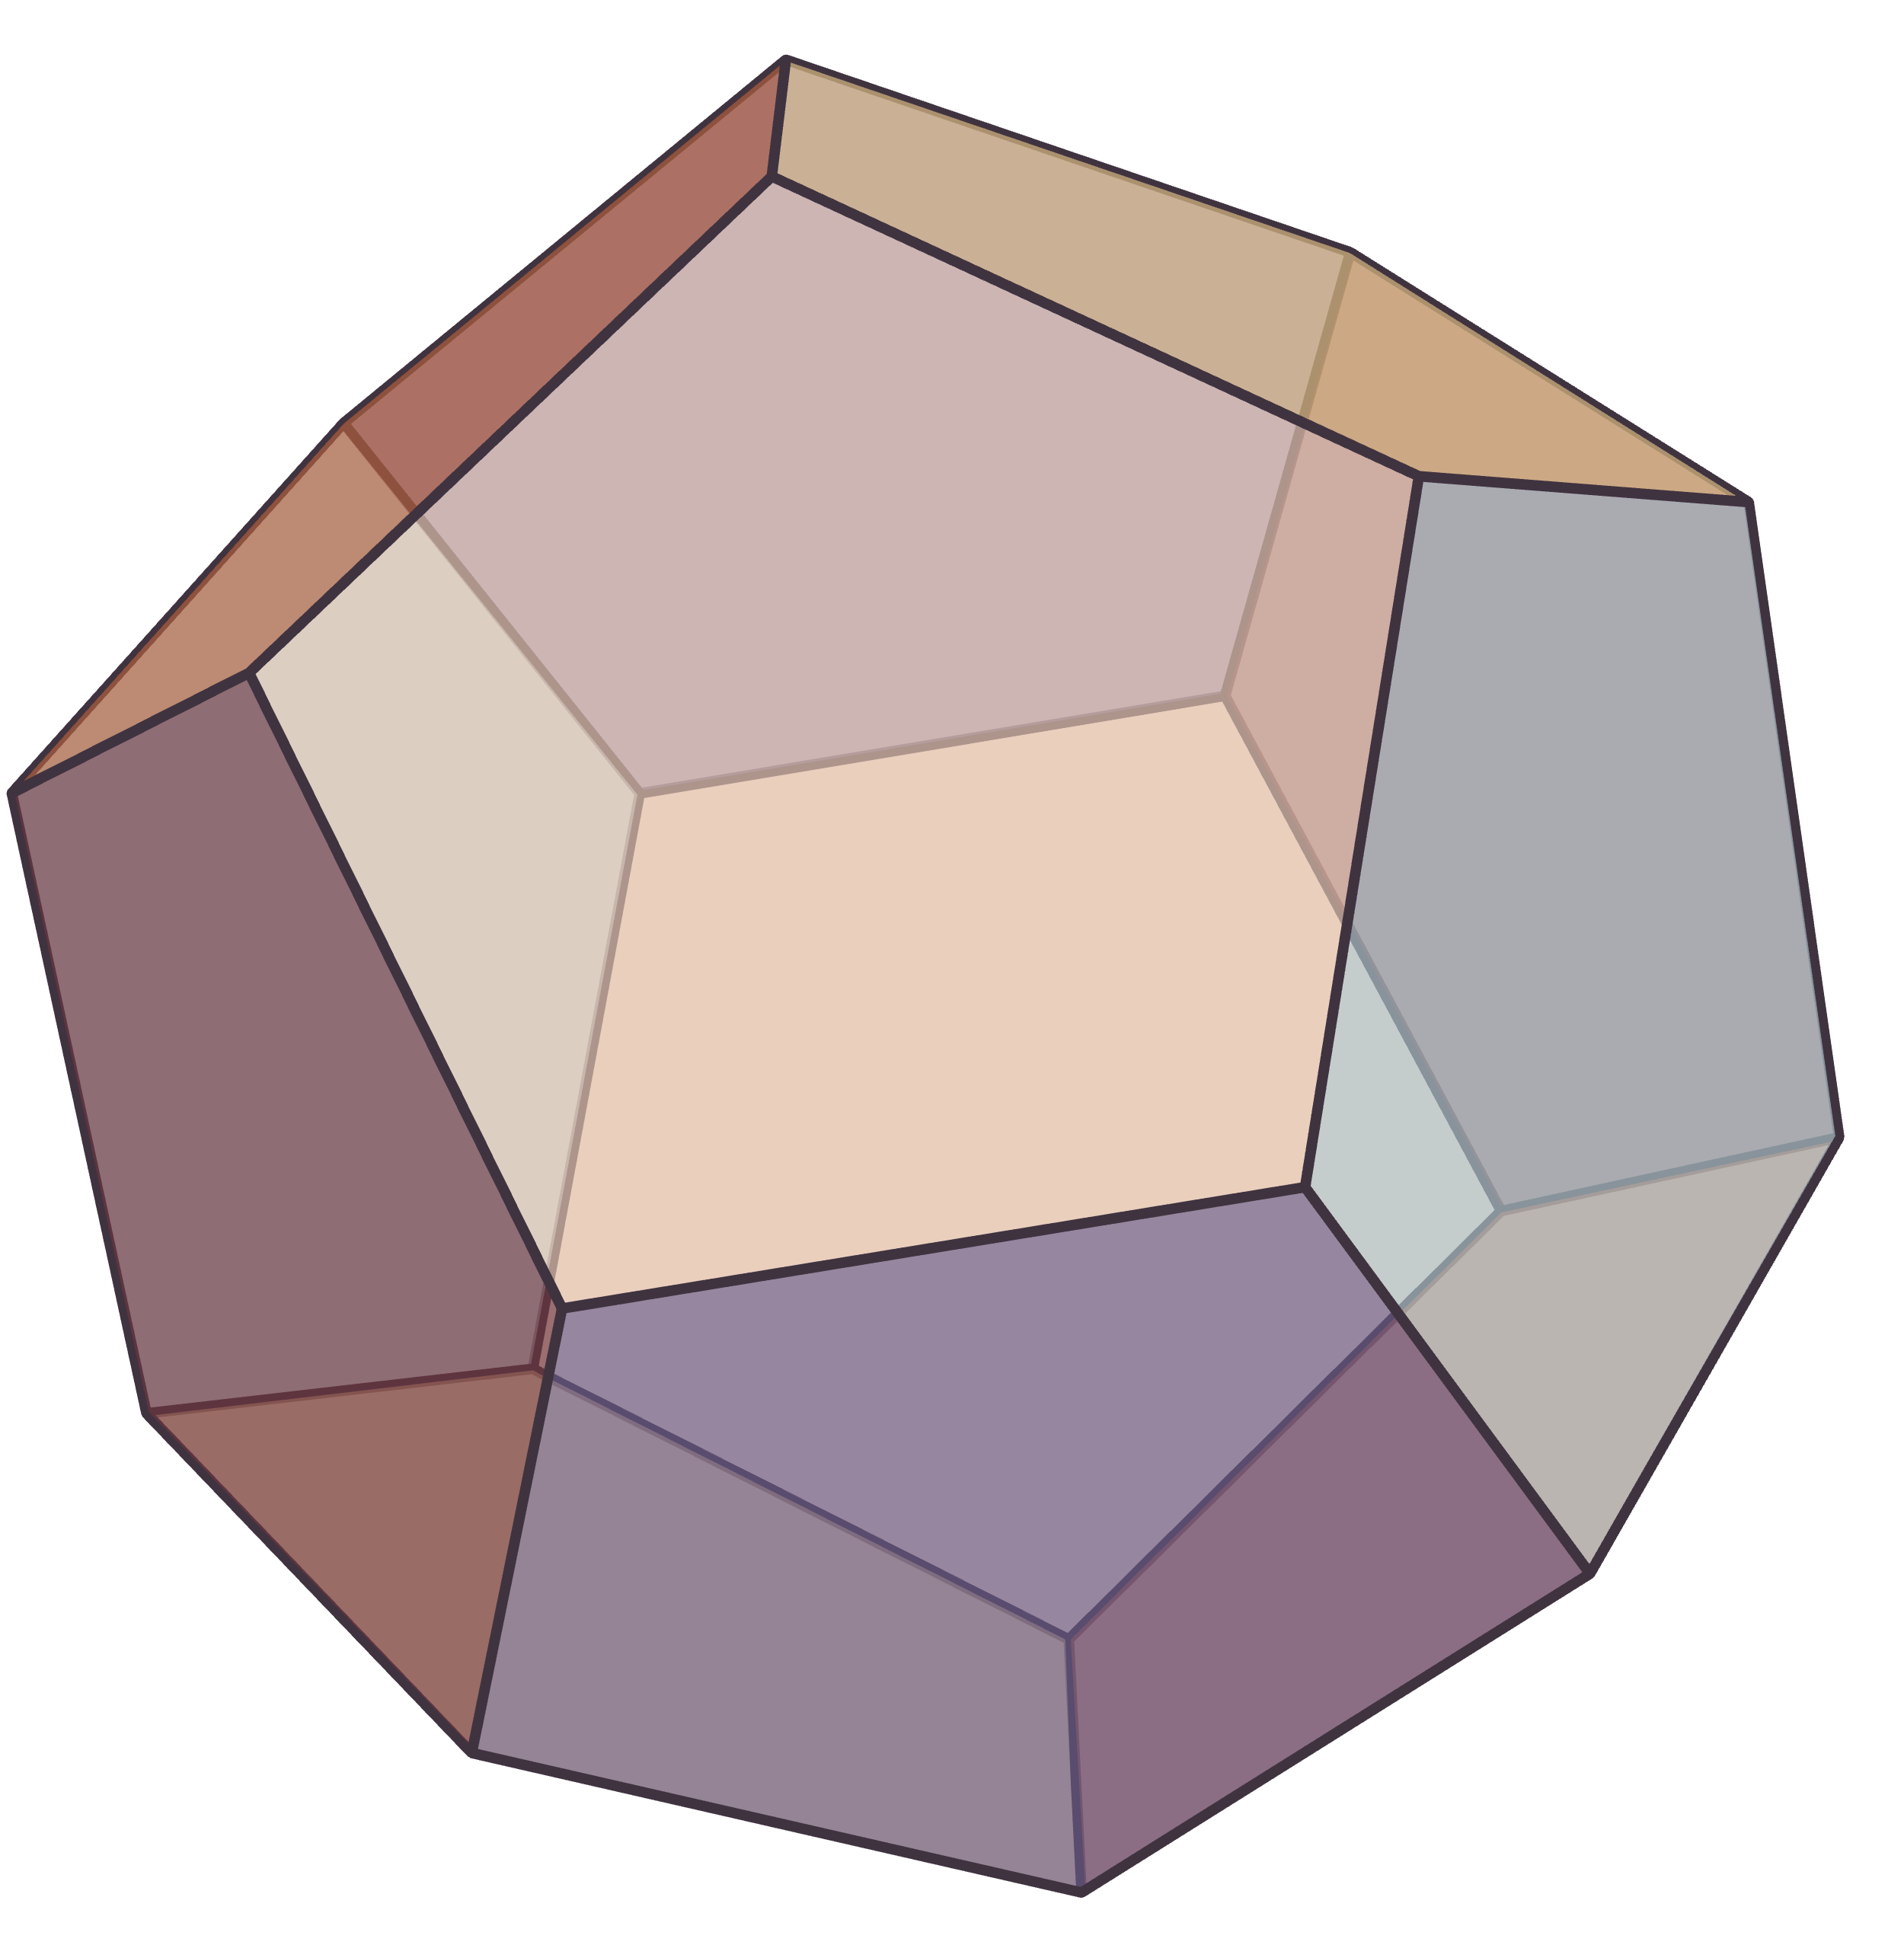
\includegraphics[height=0.1\textheight]{dodecahedron}}
    \only<1>{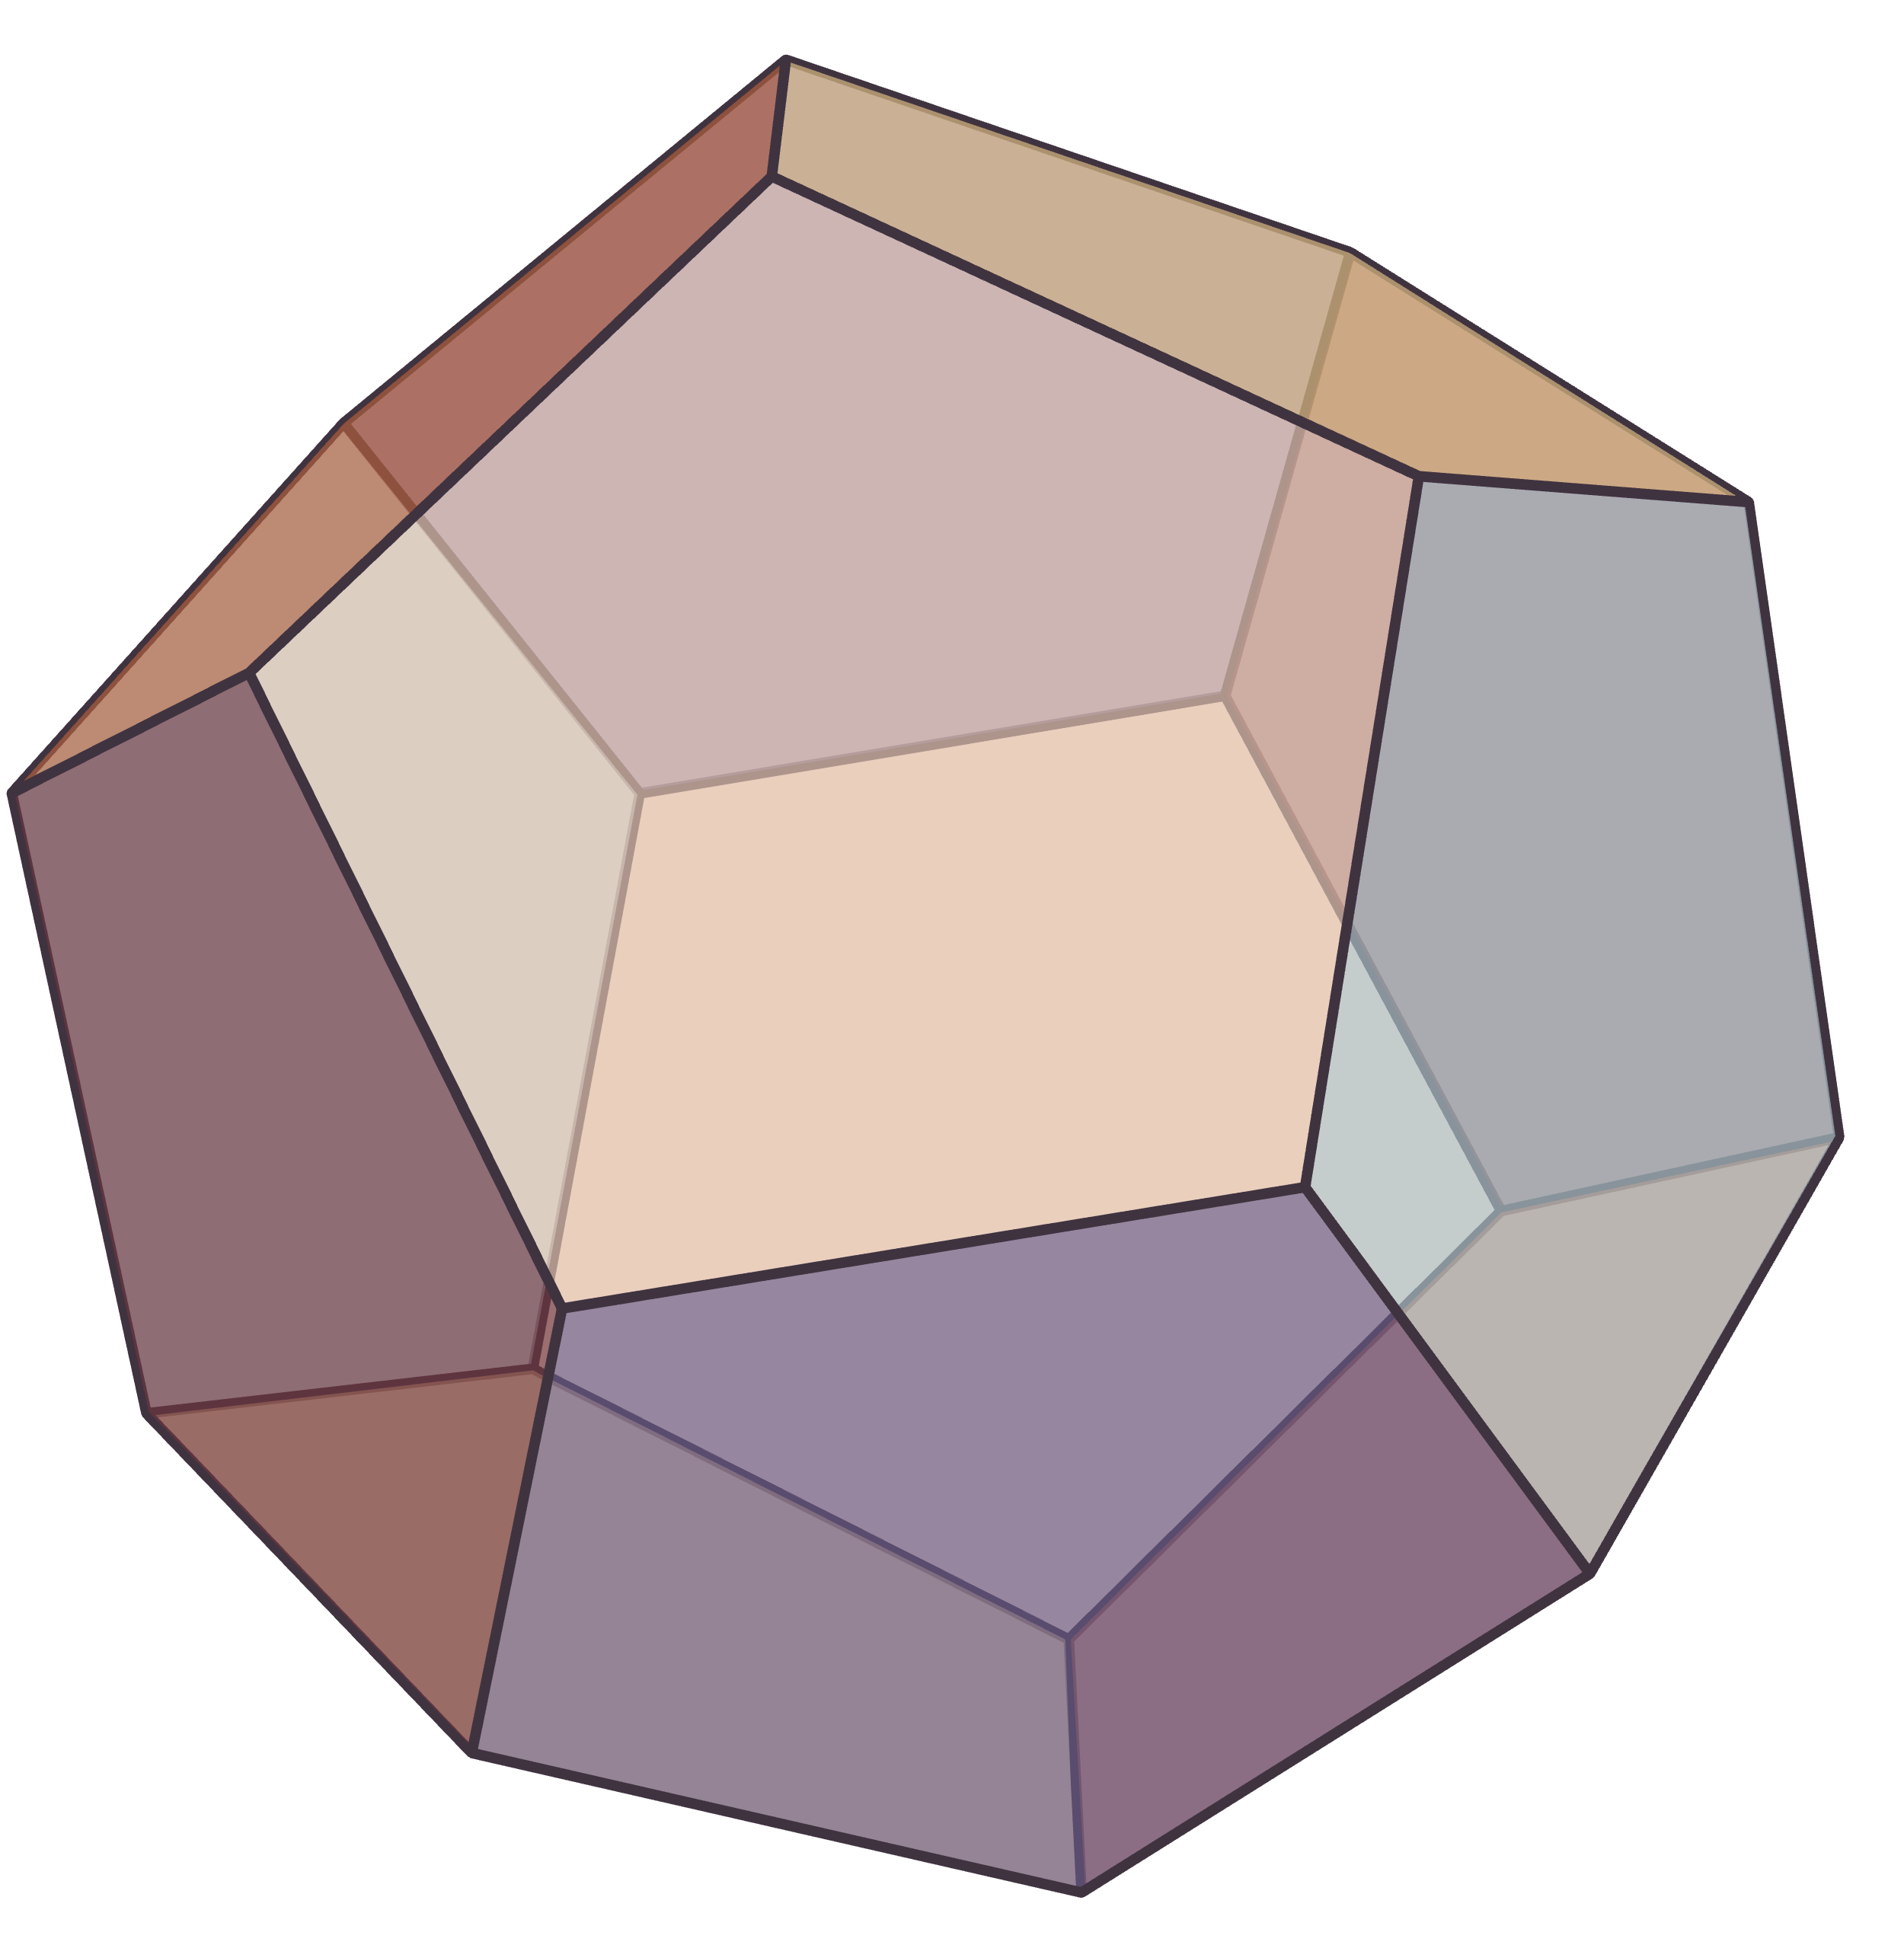
\includegraphics[height=0.7\textheight]{dodecahedron}}

    \centering
    \begin{tikzpicture}[scale=2/3]
        \only<2-9>{
            \filldraw[white,draw=black] (0,0) rectangle (6,6);
        }
        \only<3>{
            \draw[thick,dashed] (0,3) -- (6,3);
        }
        \only<4-7>{
            \draw[dashed] (0,3) -- (6,3);
        }
        \only<4>{
            \draw[thick,dashed] (0,3) -- (6,6);
        }
        \only<5-7>{
            \draw[dashed] (0,3) -- (6,6);
            \draw[dashed] (0,6) -- (6,0);
        }
        \only<5>{
            \draw[thick,dashed] (0,6) -- (6,0);
        }
        \only<6-7>{
            \draw[dashed] (0,6) -- (6,0);}
        \only<6-8>{
            \draw[thick,dashed] (0,4) -- (6,4);
        }
        \only<7-8>{
            \draw[thick,dashed] (0,2) -- (6,2);
        }
        \only<9>{
            \draw[thick,dashed] (0,4) -- (6,6);
            \draw[thick,dashed] (0,0) -- (6,2);
        }
        \only<10>{
            \filldraw[gray!15] (0,0) rectangle (6,6);}
        \only<10-12>{
            \filldraw[white,draw=black] (0,0) -- (6,2) -- (6,6) -- (0,4) -- cycle;}
        \only<13>{
            \filldraw[white,draw=black] (0,4) -- (6,2) -- (6,6) -- cycle;}
        \only<9-12>{
            \draw[dashed] (0,4) -- (6,4);
            \draw[dashed] (0,2) -- (6,2);}
        \only<13>{
            \draw[dashed] (0,4) -- (6,4);}
        \only<10-12>{
            \filldraw[gray!50,draw=black] (0,0) --++({2*atan(1/3)}:6) -- (6,2) -- cycle;
            \filldraw[gray!50,draw=black] (6,6) --++({180+2*atan(1/3)}:6) -- (0,4) -- cycle;
        }
        \only<11>{
            \draw[dashed,thick] (0,4) -- (6,2);
        }
        \only<12>{
            \filldraw[gray!15] (0,0) -- (6,2) -- (0,4) -- cycle;}
        \only<12-13>{
            \filldraw[gray!50,draw=black] (0,4) --++({90-3*atan(1/3)/2}:4) -- (6,2) -- cycle;
            \draw[dotted] (0,4) ++({90-3*atan(1/3)/2}:2) -- (6,2);
        }
        \only<13-14>{
            \path[name path=l2] (0,4) -- (6,6);
            }
        \only<13>{
            \path[name path=l1] (0,4) ++({90-3*atan(1/3)/2}:4) -- (6,2);
            \path[name path=l3] (6,6) --++({180+2*atan(1/3)}:6);
            \path [name intersections={of=l1 and l2,by=p1}];
            \path [name intersections={of=l1 and l3,by=p2}];
            \filldraw[gray!50,draw=black] (6,6) --(p1) -- (p2) -- cycle;
            \draw[thick,dotted] (0,4) -- (p1);
            \draw[thick,dashed] (p1) -- (6,2);
        }
        \only<14>{
            \filldraw[gray!15] (0,4) --++({90-3*atan(1/3)/2}:4) -- (p1) -- cycle;
            \filldraw[gray!15] (6,6) -- (p1)--(6,2) -- cycle;
            \path[name path=l4] (0,4) ++({90-3*atan(1/3)/2}:2) -- (6,2);
            \path [name intersections={of=l4 and l2,by=p3}];
        }
        \only<14-16>{
            \filldraw[gray!50,draw=black] (0,4) -- (p1) -- (6,2) -- cycle;
            \draw[dotted] (p3) -- (6,2);
        }
        \only<15>{
            \node [fill=myViolet,inner sep=1pt] at (p3) {};
            \node [fill=myViolet,inner sep=1pt] at (6,2) {};
            \path[name path=l5] ($($(p3)!.5!(6,2)$)!0.5!90:(6,2)$)--($($(p3)!.5!(6,2)$)!-0.5!90:(6,2)$);
            \path[name path=l6] (p1) -- (6,2);
            \path[name path=l7] (0,4) -- (6,2);
            \path [name intersections={of=l5 and l6,by=p4}];
            \path [name intersections={of=l5 and l7,by=p5}];}
        \only<15-16>{
            \draw[thick,dashed] (p4) -- (p5);
        }
        \only<16>{
            \node [fill=myViolet,inner sep=1pt] at (p4) {};
            \node [fill=myViolet,inner sep=1pt] at (0,4) {};
            \path[name path=l8] ($($(p4)!.5!(0,4)$)!0.5!90:(0,4)$)--($($(p4)!.5!(0,4)$)!-0.5!90:(0,4)$);
            \path[name path=l9] (0,4) -- (p1);
            \path[name path=l10] (0,4) -- (6,2);
            \path [name intersections={of=l8 and l9,by=p6}];
            \path [name intersections={of=l8 and l10,by=p7}];
            \draw[thick,dashed] (p6) -- (p7);
        }
    \end{tikzpicture}

    \only<16>{\cite{verrillOrigami}}
\end{frame}
\begin{frame}
        \frametitle{References}
        \bibliographystyle{unsrt}
        \bibliography{ref}
\end{frame}
\end{document}
\begin{frame}
    \frametitle{Recap of Graphs} 
    \begin{columns}[c]
      \begin{column}{0.4\textwidth}
    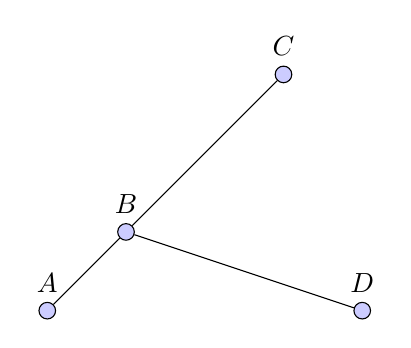
\begin{tikzpicture}
      \graph [
    nodes={
        circle,
        draw,
        fill=blue!20,      % Fills the circle with a color
        minimum size=6pt,  % Reduces the radius/size of the circle
        inner sep=0pt      % Removes internal padding so it stays small
    },
    empty nodes            % Clears the default text from inside the circles
]
{ 
    a[label=above:$A$] -- 
    b[at={(0,1)},label=above:$B$] -- 
    {
        c[at={(1,3)},label=above:$C$], 
        d[at={(2,1)},label=above:$D$]
    } 
};
    \end{tikzpicture}
          \end{column}
      \begin{column}{0.6\textwidth}
    \only<2->{
    \begin{itemize}
    \item $A, B, C, D$ are the \alert{vertices}.
    \item $AB, BC, BD$ are the \alert{edges}.
    \item The number of edges that start at a given vertex is called the \item{degree} of a vertex.
    \end{itemize}
    }
    \only<3->{
      \begin{block}{Question}
      What are the degrees of the vertices $A, B, C, D$?
      \end{block} 
    }
      \end{column}
    \end{columns}
\end{frame}


\begin{frame}
    \centering
    \begin{tikzpicture}
        \only<1>{
        \draw[very thick,fill=pink!30,rotate=45] (0,0) rectangle (4,4);
        \draw[dashed,rotate=45] (0,0) -- (4,4);
        \draw[dashed,rotate=45] (4,0) -- (0,4);}
        \only<2-3>{
        \draw[very thick,rotate=45] (0,0) rectangle (4,4);
            \draw[rotate=45] (0,0) -- (4,4);
        \draw[rotate=45] (4,0) -- (0,4);
                \draw[dashed,rotate=45] (0,2) -- (4,2);
        \draw[dashed,rotate=45] (2,0) -- (2,4);}
        \only<3>{
            \draw[->,rotate=45,xshift=2mm,yshift=-2mm] (4,0) to [out=135,in=45] (0,0); 
        }

    \end{tikzpicture}
\end{frame}